% Scalar instruction entry source: tools/generate_scalar_instruction_catalog.py.
\subsection{\texttt{B.GE}}
\label{sec:scalar-b_ge}
\index{B.GE@\texttt{B.GE}}
\begin{sloppypar}\noindent\textbf{Purpose.} Conditional branch. The branch is taken when the selected condition holds (greater-or-equal (signed)).\end{sloppypar}\smallskip
\noindent\textbf{Syntax.}\par
\begin{lstlisting}[style=ptoscalarcode]
b.ge SrcL, SrcR, label
\end{lstlisting}
\noindent\textbf{Encoding.}\par
\noindent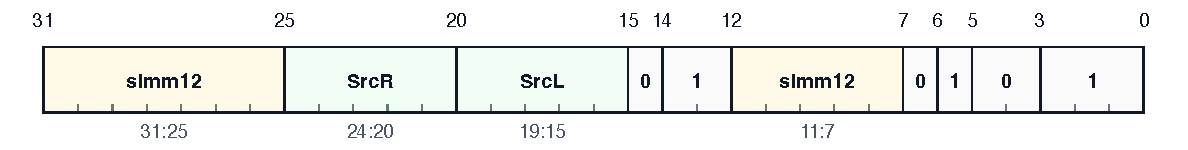
\includegraphics[width=\textwidth]{figs/encoding/scalar_instruction_entries/enc_b_ge.pdf}\par\smallskip
\begin{description}[leftmargin=0.18\linewidth,style=nextline]
\item[Format] \texttt{L32} \texttt{32-bit} scalar word.
\item[Pattern] \texttt{.................011.....0100111}.
\end{description}
\noindent\textbf{Classification.}\par
\begin{description}[leftmargin=0.18\linewidth,style=nextline]
\item[Category] Branch, Compare, and PC Control.
\item[Family] Branch.
\item[Execution class] \texttt{BRU}; uop\_kind=BRU.
\end{description}
\noindent\textbf{Operand fields.}\par
\begin{description}[leftmargin=0.18\linewidth,style=nextline]
\item[\texttt{SrcL}] Bits \texttt{19:15 (5b)}. 5-bit scalar source register used as the left operand of the branch condition.
\item[\texttt{SrcR}] Bits \texttt{24:20 (5b)}. 5-bit scalar source register used as the right operand of the branch condition.
\item[\texttt{simm12}] Bits \texttt{31:25 (7b), 11:7 (5b)}. 12-bit signed PC-relative branch displacement. The decoded offset is sign-extended and added to the current PC when the condition is true. The immediate is split across non-contiguous encoding slices and reassembled before use.
\end{description}
\noindent\textbf{Operation.}\par
\begin{lstlisting}[style=ptoscalarcode]
if (Read(SrcL) >= Read(SrcR)  // signed):
  TPC = <target>
\end{lstlisting}
\Needspace{0.08\textheight}
